%==============================================
\subsection{Ranking of Frontier Gaps}\label{subsec:gap}

When the condition in~\eqref{eq:wccg_criterion} fails, the vehicle cannot
reach~$\mathbf{x}_\texttt{V}^{\texttt{G}}$ from
$\mathbf{x}_\texttt{V}^{\texttt{S}}$ through a~$W$--clear path
$\mathcal{P}^W_\texttt{V}$.
In this case, the planner must prioritize
\emph{blocking gaps} on the reachable frontier of~$\mathcal{G}_W$
according to their predicted downstream cost, and feed the ranked list to the
hybrid search as local clearance targets.

\subsubsection{Frontier Extraction and Candidate Gaps}
A BugPlanner query on~$\mathcal{G}_W$ above
either confirms connectivity or returns a counter--clockwise frontier loop
$\mathcal{L}$ that separates the two endpoints. The bridge--bridge edges on
$\mathcal{L}$ define the first--hop candidate set
$\Gamma_\mathcal{L}\triangleq\{g_1,\cdots,g_K\}$,
where each gap~$g_k$ is represented by its two closest boundary points, its
width~$w_{g_k}<W$, and the adjacent obstacles that can potentially be moved.
These candidates are then ranked by predicted downstream cost and passed to the
hybrid search as local clearance targets.

\subsubsection{Evaluation for Immediate Cost}
Each candidate~$g\in\Gamma_\mathcal{L}$ is evaluated by combining the
cost for the robots to reach the gap and the effort required to widen it.
Let~$\mathbf{s}_{\mathcal{R}}$ be the current robot positions,
and~$\mathbf{o}_g$ as the outside insertion point of gap~$g$. The
resulting one--hop cost is given by:
\begin{equation}\label{eq:step_cost}
\mathsf{C}\big(g \mid \mathcal{L}, \mathbf{s}_{\mathcal{R}}\big)
=\lambda_\texttt{t}\,\mathsf{C}_\texttt{t}\!\left(\mathbf{s}_{\mathcal{R}},\mathbf{o}_g\right)
+\lambda_\texttt{p}\,\big( \mathsf{C}_\texttt{dp}(g) + \mathsf{C}_\texttt{rp}(g)\big)
\end{equation}
where~$\lambda_\texttt{t},\lambda_\texttt{p}>0$ weight transition and pushing costs, respectively; $\mathsf{C}_\texttt{t}$, $\mathsf{C}_\texttt{dp}$, and $\mathsf{C}_\texttt{rp}$ denote transition, direct-pushing, and recursive-pushing costs.

%------------------------------
\begin{figure}[t!]
  \centering
  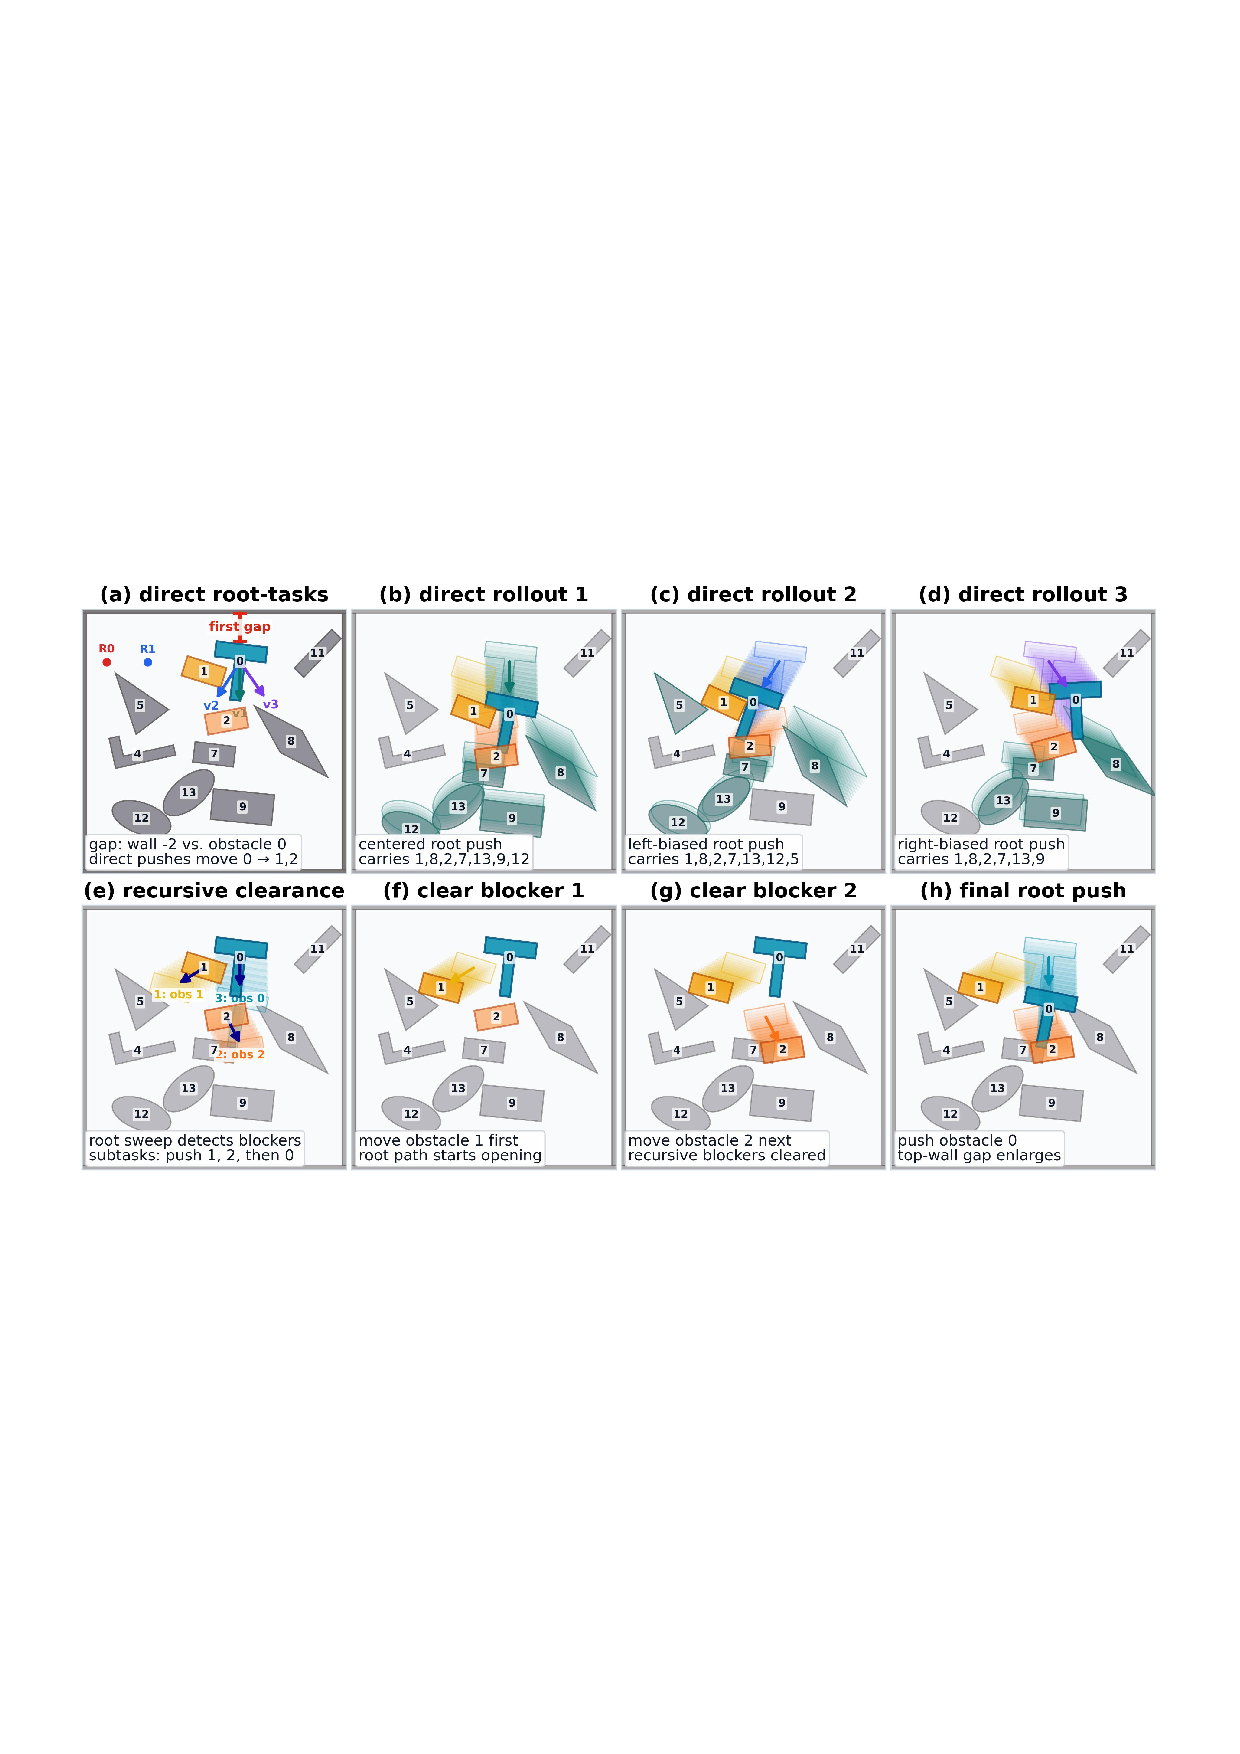
\includegraphics[width=0.82\linewidth]{figures/direct_recursive_push.pdf}
  \vspace{-0.1in}
  \caption{\change{
  \textbf{Direct} pushing moves a gap-side blocker along a gap-opening direction,
  whereas \textbf{recursive} pushing first clears movable blockers in the swept
  region and then returns to the root gap-opening task.}}
  \label{fig:direct_recursive_push}
  \vspace{-4mm}
\end{figure}
%------------------------------

\subsubsection{Long-term Cost w.r.t. Goal}
Furthermore, to prioritize gaps closer to the goal, a heuristic is added to the evaluation,
i.e.,
$h(g)=\eta\,\big\|\mathbf{o}(g)-\mathbf{x}_\texttt{V}^{\texttt{G}}\big\|$,
with the scaling constant~$\eta>0$.
Lastly, a short A$^\star$-style presearch is adopted to cross
each candidate gap, recompute the next frontier, and continue for a limited
width and depth. The \emph{cost-to-connect} is predicted by:
\begin{equation}\label{eq:pred_cost}
\widehat{\mathsf{Cost}}(g)\triangleq
\mathsf{C}\!\big(g \mid \mathcal{L},\mathbf{s}_{\mathcal{R}}\big)
+\!\!\!\sum_{g'\in\Pi^\star(g)}\!\!\!\big{\{}\mathsf{C}(g' \mid \cdot)+h(g')\big{\}},
\end{equation}
where~$\Pi^\star(g)$ is the sequence of subsequent gaps discovered after virtually crossing~$g$. Consequently, the final output of this module is the ranked list of candidate gaps, i.e.,
$\textsf{Rank}\big(\Gamma_\mathcal{L}\big)
\triangleq \textbf{argsort}_{g\in\Gamma_\mathcal{L}}\widehat{\mathsf{Cost}}(g)$,
in ascending predicted cost. This
ordered set is passed to the hybrid search module, such that only the
promising gaps are expanded first.


